	
	\section{Dark Silicon}
		\subsection{Obituary for Moore’s Law and Dennard Scaling}
			The origin of Moore's Law stems from a paper released in 1965, titled \textit{Cramming more components onto integrated circuits}. In this paper, Moore predicted the number of transistors in an integrated circuit would double every 18-24 months \cite{BookOfMoore}. This relationship was representative of trends in computer development until round the mid 2005. Figure~\ref{SRAMGraph} shows trends on the spacing of components on chips, and as can be seen the trends slows down around the 2005-2010 mark.	Around the same time, Dennardian Scaling was experiencing a similar downfall.
			
			In 1974, Robert H. Dennard et al. released a paper titled \textit{Design of ion-implanted MOSFET's with very small physical dimensions}, in which he observed the relationship between transistor size, frequency, capacitance and and operating voltage $V_{DD}$. He found that for fixed power and area budgets, an exponential increase the maximum number of transistors that will fit into the area results in a linear increase in maximum operating frequency \cite{SmallDimensionMosfets}. This can be seen in Figure~\ref{DennardianScalingTable},and is termed Dennardian Scaling. A 33 year review of Dennard et al. in 2007 found that the assumptions that underpinned Dennardian scaling were inadequate. For example, it was assumed that MOSFET channel doping concentrations would continually increase, producing shorter channels with each generations. In reality, it was found that as the concentration of channel doping increases, impurity scattering caused the carrier performance and mobility to degrade. A number of Dennards assumptions failed, and this resulted in Post-Dennardian Scaling, which can also be seen in Figure~\ref{DennardianScalingTable}, where the operating voltage has ceased to decreased with transistor size and so the power requirements of new generating are exponentially increasing. Conversely, we see on chip utilisation for a fixed power budget decreases exponentially.\cite{ReviewOfDennard}.
			

			\begin{figure}

				\begin{center}
					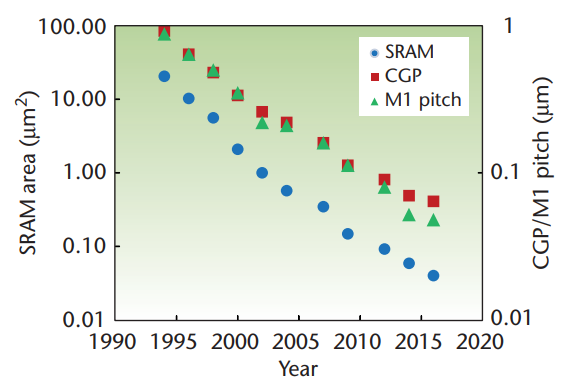
\includegraphics[width=0.5\textwidth]{SRAM CGP and M1 Pitch Graph.png}
				
				\caption{Historical data from the last 20 years of chip development \cite{TheEndOfMooreTheis}.}
				\end{center}
				\label{SRAMGraph}
			\end{figure}
		
		
			\begin{figure}
				
				\begin{center}
					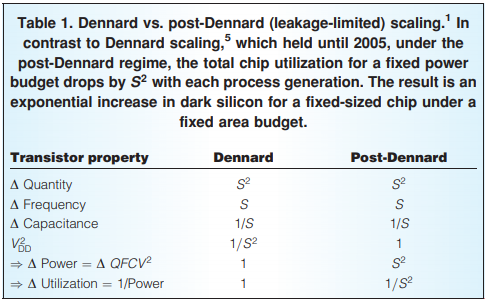
\includegraphics[width=0.5\textwidth]{Dennardian scaling table.png}
					
					\caption{Ratios in Dennardian and Post-Dennardian Scaling. \cite{TheEndOfMooreTheis}.}
				\end{center}
				\label{DennardianScalingTable}
			\end{figure}
			
		\subsection{The minimum energy for computing}
		
			In the 20th century, Charles H. Bennet et al. proved that for any irreversible computation there is a minimum amount of switching energy required, equivalent to $k|{B}T\ln{2}$, where k is the Boltzmann constant, and T is the temperature. At room temperature this is approximately $10^{-21}$J, or 1 zeptojoule. This limit is called the Shannon-von Nuemann-Landauer limit and it is descriptive of switching elements' physical properties, specifically that the lower power limit for their function is very low. The relevance of this is thus: a driving factor in dark silicon is that as transistor size reduces, transistor power usage still reduces. Though the new trend of increating power density is linked to decrease in transistor size, transistors are not the limiting factor. The limiting factor is that transistors are no longer the primary source of energy consumption \cite{MinEnergyInComputing}.
			
			The primary source of energy consumption in embedded electronics is electrical capacitances. In integrated circuits, the most common forms of capacitance are wire interconnects. Short interconnects are modelled as capacitive lumps in the circuit, while medium length interconnects are modelled as lossy RC transmission lines and long interconnects are modelled as lossy RLC transmission lines. As transistor size scales down, these interconnects are becoming the dominant limitation for clock frequency, power utilisation and transmission delay in-circuit.
			
			In contemporary microprocessors in the 22-65nm range, the total energy consumptions attributed to transistors makes up only ~20-30\% of the total energy budget. This percentage is expected to decrease as transistor size decreases \cite{MinEnergyInComputing, Interconnects}. 
		
		
		
		
		\subsection{The Four Horsemen of Dark Silicon}
			As we move into an era of CPU design defined by Post-Dennardian Scaling, we must address the exponential decrease in chip area utilisation. This decrease has a significant effect on multicore scaling, as fitting more cores onto chip requires those cores to be under-clocked, underpowered, or not powered at all. In an article titles \textit{The Four Horsemen of Dark Silicon}, Michael B. Taylor categorised the primary methods for resolving the dark silicon problem. He refers to them as the "4 Horsemen", and ordered from most to least relevant they are:
			
			\begin{itemize}
				\item \textbf{The Specialised Horseman} - Heterogeneous core design.
				\item \textbf{The Dim Horseman} - Under-clocked or underpowered cores. 
				\item \textbf{The Shrinking Horseman} - Reduced area core design.
				\item \textbf{The Deus Ex Machina Horseman} - Material science advancements.
			\end{itemize}
		
			\subsubsection{The Specialised Horseman}
				A typical ASIC circuit is usually 100 to 1000x faster than a general processing unit, as well as 157 to 707x more energy efficient for a given task \cite{InefficiencyInGeneralPurposeChips}. While achieving these levels or performance and power efficiency is unlikely in a general processing unit, attempting to imbue a softcore with these properties would, if successful, produce a core that performs tasks faster, with a lower power budget, at the cost of an expanded area requirement. Dark silicon leaves us with a surplus of space and a deficit of power, making design choices that trade expanded circuitry for minimized power budgets ideal \cite{DarkSideOfSilicon, TheFourHorsemen}.
				
			\subsubsection{The Dim Horseman}
				A cousin of dark silicon is dim silicon. Dim silicon refers to under-clocked or underpowered sections of the chip. By reducing the voltage or frequency, the power budget can be met. For example, Figure~\ref{DimSilicon} shows a an example dim silicon implementation, with an increase in core numbers but no increase in clock frequency. Dynamic Voltage and Frequency Scaling are dim silicon methodologies and DFS is of interest to this project, as it can be implemented in an FPGA using controlled prescalers.
				
				Computation sprinting is a form of DFS where the chip spends most of its time in an under-clocked state, and spends short bursts or "sprints" in at a higher clock rate that produces excessive heat on chip. Once the heat reaches a safety-limit, the chip is returned to a low clock rate, and the heat is allowed to dissipate. This allows for a balance while managing energy and thermal considerations. This method can be implemented in a multicore system \cite{ComputationalSprinting}.
				
				Underpowered silicon involves running sections of the chip at a lower voltage than the transistors are rated for, the power budget can be reduced in exchange for an increased risk of metastability. This is called Near Threshold Voltage processing. This method is out of scope for this project, for the same reason as DVS \cite{DVS}.
				
				\begin{figure}
					\centering
					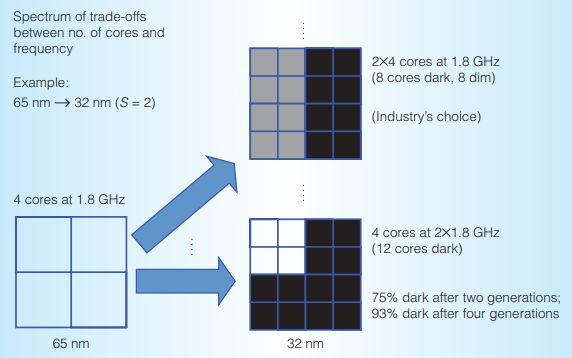
\includegraphics[width=0.7\textwidth]{DimSilicon.png}
					\caption{text}
					\label{DimSilicon}
				\end{figure}
			
			\subsubsection{The Shrinking Horseman and the Deus Ex Machina Horseman}
				The Shrinking Horseman refers to what I have termed reduced area design. The design methodology is in the label: shrink the size of CPU's and use smaller die. By simply removing the dark silicon from the chip, the problem is neatly sidestepped. This solution is not in the scope of this project.
				
				The Deus Ex Machina Horseman refers to the aforementioned advances in material design. Again, the method is in the label: a god-out-of-the-machine event might remove the constraints of dark silicon by increasing the allowable power budget a CPU can handle, or by decreasing the power budget required for modern computing. Already scientists are experimenting with different semiconductor substrates, 3 dimensional chip designs and photonic interconnects, each of which could resolve the dark silicon problem. Photonic interconnects in particular could be extremely efficient as a solution to the problem of lossy RC and RLC interconnects. Nonetheless, this is the realm of material scientists and is outside of the scope of this project \cite{TheFourHorsemen}.
			
		\subsection{Memory Driven Computing}
			Memory Driven Computing is an attempt to deal with the power constraints caused by interconnects. In a standard computers, memory is stored in multiple units at varying distances from the computing unit. The closer the memory units is to the CPU, the less memory it can hold. This varied memory model is used because the memory closer to the CPU tends to be more expensive per bit, in a relationship described in Figure~\ref{StorageDeviceHierarchy}.
			
			\begin{figure}
				\centering
				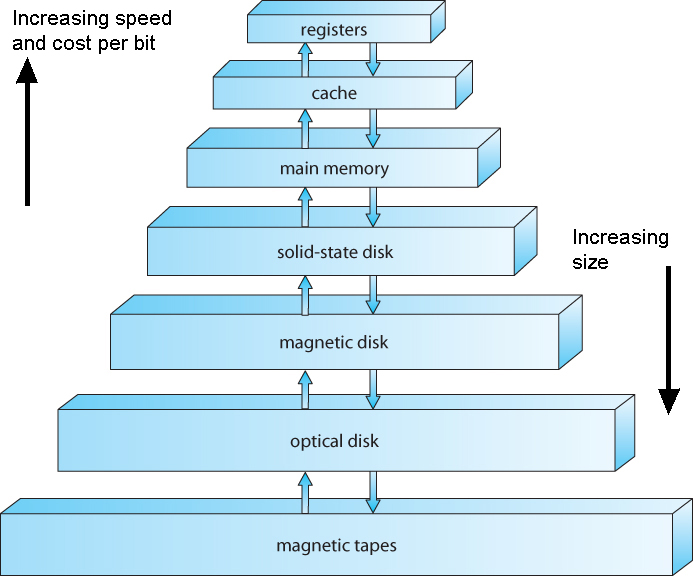
\includegraphics[width=0.5\textwidth]{StorageDeviceHierarchy.jpg}
				\caption{Computer Memory System Model \cite{CPUScheduling}}
				\label{StorageDeviceHierarchy}
			\end{figure}
		
			A similar principle at chip level is used in placing cache memory: it is often located on one section of the chip, with the core or cores elsewhere. This can lead to large interconnects required to join the memory with the core or cores. Memory Driven Computing seeks to distribute cache memory around the chip, specifically to be close to the core or cores, reducing the number of large interconnects on the chip required to move memory around \cite{EndOfMooresLawWilliams}. 
		
		\subsection{The Dark Side of Silicon}
			In 2017, Rahmani et al. released a book title \textit{The Dark Side of Silicon}, spanning a collection of works in the dark silicon research space. This book is a fountain of information for dark silicon design methodologies, and outlines a combined hetergeneous methodology and memory driven computing methodology that inspiration is drawn from.\\
			The SiLago methodology was developed to remedy the following issues in CPU design:
			\begin{itemize}
				\item Most design focuses on cores, ignoring memory and inteconnects
				\item Software layer abstractions often employ naive resource allocations, which results in runtime inefficiencies.
				\item A absence of dynamic customization at runtime means that non-deterministic concurrency and communications patterns produce power usage and parallelism inefficiencies.
				\item Over-customisation is prohibitive due to large engineering costs.
			\end{itemize}
			The SiLago methodology answers these problems by implementing a distributed memory architecture. This directly combats losses from interconnects and has been shown to significantly reduce power and energy expenditure on chip when properly implemented \cite{SiLagoSolution}. Similar methodologies have shown that arbitrarily placing memory through the chip significantly reduced the power losses from on-chip interconnects \cite{DynamicDirectories}.
	
	\section{Task Scheduling}
		
		\subsection{Algorithms}
			The aim when scheduling for CPU's is to maximum resource allocation usually by pausing a program while it waits for a I/O or system call commands to return. Scheduling attempts to maximise CPU utilisiation, data throughput, task turnaround time, task waiting time (time spent waiting on I/O or systems calls, etc.) and task response time (how long a task waits in the queue before reaching the CPU).
			
			Priority scheduling approaches this by assigning tasks different priorities. This ensures that the most important tasks aren't blocked by less important tasks, though it can result in less important tasks being blocked for extended periods. A solution to this is a Multilevel Feedback Queue, which uses multiple queues to designate tasks that have been waiting or running for different periods of time. It ensures that priority is given to the most relevant tasks, whilst also preventing less important tasks from being ignored \cite{CPUScheduling}.
		
		\subsection{Variation Aware Core Selection}
		 	In conjunction with heterogeneous core implementation, there is the scheduling methodology called Variation Aware Core Selection. This methodology utilises the heterogeneous nature of an implementation to schedule tasks to the core best suited for their workload. This fusion between good hardware design is an example of the way to get the best performance out of chips by utilising an ASIC like implementation. Without the variation aware resource allocation, the heterogeneous implementation would be wasted. \cite{HeterogenousCoreDesign}.
			
		
	
	\section{Thermal Considerations}
		\subsection{Thermal Hotspots}
			Heat distribution on chip is non-uniform and non-trivial. Their are a number of temperature gradient that exist across the chip, typically described by a number of hotspots on the chip. Hotspots present an issue wherein a localised section of a chip risks damage. The distribution varies with workloads, and differs between die due to physical variations (e.g. thickness of substrate), and in a multicore system this distribution is an product of the interactive heat dissipation from the different cores. As shown in Figure ~\ref{fig:DieHotspots}, hotspots tend to arise in the regions of the die allocated for cores, though they arise in a variety of function units, such as I-cache, D-cache or floating point units. The tendency of a region to become a hotspot is workload dependent.  . 
			
			\begin{figure}[h]
				\centering
				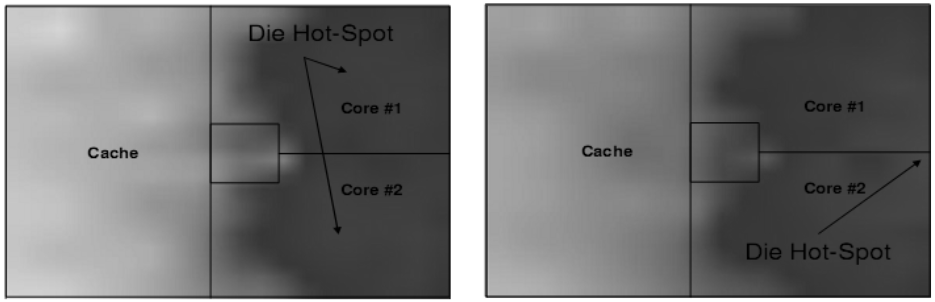
\includegraphics[width=0.7\textwidth]{DieHotspots.png}
				\caption{Heatmaps of local hotspots on a multicore die under different workloads \cite*{HotspotsInDie}}
				\label{fig:DieHotspots}
			\end{figure}
		
			A hotspot acts a pole for temperature. The heat dissipation around this pole can be modelled using the formula 
			\begin{equation}
				T(x,t) = \frac{Q}{2 \pi \lambda x} \left[ 1-\frac{2}{\sqrt{\pi}} \sum_{n=0}^{\infty} (-1)^n \frac{r^{2n+1}}{\prod_{n=1}^{n}n(2n+1)}) \right]
			\end{equation}
			which in steady state, as $t \to \infty$, becomes equivalent to 
			\begin{equation}
				T(x) = \frac{Q}{2 \pi \lambda x}
			\end{equation}
			As the dimensions of the die decrease, if a heat-naive layout is maintained, the dissipation areas around the hotspots overlap, putting sectors between hotspots at risk of degradation. Layout that herd hotspots into each other proximity create temperature bottlenecks for temperature that reduces the quality of temperature dissipation across the chip for all hotspots. The solution to combat this is the distribute likely hotspots across the chip, giving them a larger area around themselves to dissipate heat.
			
			In particular, several software methods utilise this approach by apportioning workloads to different function units in the die. These methods reduced the hotspot temperatures and the average temperature across the die \cite*{HotspotsInDie}.

		\subsection{Dynamic Thermal Management and Hotspot Management}
			Dynamic Thermal Management (DMT) is emerging as an alternative to traditional solid state thermal management. The goals is to make cooling routines adaptive to the circumstances to make them more effective. Particularly of interest here is DTM with regards to hotspot management. While hotspot remediation is still progressing as a field, several examples of it are cropping up and they present opportunities in the land of dark silicon. For example, Bar-Cohen et al. experimented with using Mini-Contact Enhanced Thermo-Electric Coolers, In-Plane Silicon Microcoolers, Si/SiGe Superlattice Microcoolers and Microgap coolers, and found they could reduce hotspot temperatures by as much as 17$^{o}$C, in the context of a hotspot 37$^{o}$ hotters than surrounding silicon \cite{Bar-CohenAvram2012Tmoo}.
			

		\subsection{Thermal Aware Design}
			Thermal aware design is a CPU implementation method that takes cooling procedures into account. Fully realised thermal aware design involves tailoring thermal management of the CPU as well, which is out of the scope of this thesis. A key consideration is that thermal aware designs do not necessarily translate well between different chips. So, thermal aware considerations in this project come with the assumption that these design will be possible in the future. The practical thermal management is out of the scope of this project, but utilising thermal management in the context of hotspot management fits neatly into the dark silicon ballpark. Appropriate thermal aware design can produce considerable improvements in efficiency over non-thermal aware design methodologies, so it is worth designing chips with the capacity to employ thermal aware methodologies in the future \cite{ThermalAwareDesign, ThermalSafePower}.
	
	\section{RISC-V}
		\subsection{The RISC-V ISA}
			The RISC-V ISA is a reduced instruction set architecture. It is useful in an open source context as it comes in multiple bit-lengths and is entirely modular. The base instruction set contains standard logic flow control functions, standard IO and addition and subtraction. Additional modules add functionality for multiplication and division, atomic functions, floating point operations, control status register implementation and more. The full outline can be found in \textit{The RISC-V Instruction Set Manual Volume I: Unprivileged ISA} \cite{riscvUnprivIsa, riscvPrivIsa}.
		\subsection{RISC-V Cores}
			Different cores implement different levels of the RISC-V ISA. For the sake of later discussion, the following warrant mention:
			\begin{itemize}
				\item \textbf{RISC-V Processing UNIT (RPU)} implements the base instruction set and the control status register instruction set in 32-bit architecture.
				\item \textbf{InstantSOC} implements the base instruction set and the multiplication instruction set in 32-bit architecture.
				\item \textbf{VexRiscv} implements the base instruction set, the multiplication set and the control and status register instruction set in 32-bit architectures \cite{riscvCores}.
			\end{itemize}
			
		